\documentclass[10pt,conference,letterpaper]{IEEEtran}
\usepackage{graphicx}
\usepackage{soul}

% pete's adds
\usepackage{color}
\newcommand{\todo}[1]{{\textcolor{red}{#1}}}
\newcommand{\blue}[1]{{\textcolor{blue}{#1}}}
\newcommand{\pjk}[1]{[\todo{PJK: #1}]}

\newcommand{\pjkst}[2]{[\todo{PJK: #1}]\st{#2}}
\newcommand{\note}[1]{\textcolor{blue}{[#1]}}
\newcommand{\red}[1]{\textcolor{red}{#1}}

\begin{document}
\title{Federated Consistency in Geographically Distributed Systems}
\author{\IEEEauthorblockN{Benjamin Bengfort and Pete Keleher}
\IEEEauthorblockA{Department of Computer Science\\
University of Maryland, College Park, MD, USA\\
\{bengfort,keleher\}@cs.umd.edu}}


\date{December 12, 2016}

\IEEEtitleabstractindextext{%
\begin{abstract}
Consistency in a distributed storage system is usually thought of as one of a few discrete categories: eventual, causal, sequential, or linearizable and distributed systems are designed with homogenous replica types to fit one of those categories. In this paper we present Federated Consistency, a heterogenous system model that allows individual replica servers to select their own consistency level, specifying a quality of service at a particular location while still providing global guarantees. This model, applied to variable latency geographic systems that are partition prone allow for flexibility in consistency that can adapt in response to the local network environment.
\end{abstract}}

\maketitle

\IEEEdisplaynotcompsoctitleabstractindextext

\section{Introduction}

The rise of on-demand computing resources and the Cloud have made distributed systems the default approach to scaling applications for many users in a variety of geographic locations. In particular, data replication is used to increase availability, throughput, durability, and fault tolerance by ensuring that objects can be accessed on multiple servers as locally as possible. Although some coordination is necessary to ensure that replication happens correctly, many systems favor a relaxation in consistency in order to meet the performance requirements of modern, mobile applications. This is partially because the application layer can define its own mechanisms for handling differently consistent behavior but it is primarily because such systems are implemented in data center contexts that enjoy stable, low-latency connections which allow optimistic approaches and provide consistent views of data \emph{most of the time} \cite{bailis_quantifying_2014,bermbach_metastorage:_2011}.

We might, therefore, generally categorize most modern distributed storage systems and NoSQL databases as not having strong consistency and using some consensus algorithm for control and synchronization when necessary. As a result consistency is usually described in a discrete, data-centric fashion: weak or strong; eventual, causal, or sequential and no longer described in client-centric terms \cite{bermbach_consistency_2013}. As replication becomes more prevalent, however, it is not enough to simply lay the burden of conflict at the feet of clients and there has been recent interest in instead redefining consistency along a spectrum whose dimensions are the strictness of ordering writes and the potential staleness of reads \cite{yu_design_2002,li_making_2012,afek_quasi-linearizability:_2010,al-ekram_multi-consistency_2010,krishnamurthy_adaptive_2002}.

By defining consistency in terms of ordering and staleness it is easy to see that the root cause of the tradeoff between performance and correctness is message latency, where a common case is when messages do not or cannot arrive due to node failure or network partitions. It has been noted that message latency is the key factor in determining ``how consistent'' a system is either due to staleness in eventually consistent systems \cite{bailis_probabilistically_2012} or by preventing progress in sequential consistency systems implemented with consensus \cite{howard_raft_2015}. The advent of distributed storage as a service has allowed systems to adapt consistency at runtime by taking advantage of a stable network environment \cite{chihoub_harmony:_2012,chihoub_consistency_2013,kraska_consistency_2009} and has shifted the focus away from replication in weakly-connected, dynamic, or mobile networks even though it is the environment that has the primary role in determining the behavior of replication and potential guarantees \cite{pitoura_data_1999,deno-toc}. \pjk{Important...}We believe that local, user-oriented distributed systems should augment cloud services rather than be replaced by them; and in some cases, such as disaster recovery or search and rescue, may be the only available system.

In this paper we present a novel approach to flexible consistency via the federation of a heterogenous system of replica servers that implement a variety of consistency protocols in response to local policies and requirements. As a result, individual replicas in the system can respond and adapt to a changing network environment while providing as strong a local guarantee or minimum quality of service as required. The global state of a federated system is defined by the topology of replicas and their interactions, such that if a subset of nodes implement stronger consistency models, then the global probability of conflict is reduced and conversely if a subset of nodes implements weaker consistency then global throughput is increased. Indeed, we find that it is more often the tension between local vs global views of consistency that cause greatest concern in terms of application performance. Because each node can select and change local consistency policies, client applications local to the replica server have greater control of tuning consistency in response to mobile or dynamic network behavior, maximizing timeliness or correctness as needed.

We show that a federated consistency protocol finds a middle ground in the trade-off between performance and consistency, particularly between an eventually consistent system implemented via gossip-based anti-entropy \cite{kempe_gossip-based_2003} \pjk{HAT...} and a sequential consistency model implemented by the Raft consensus protocol \cite{ongaro_search_2014}. By exploring these two extremes in the consistency spectrum we show that the overall number of inconsistencies in the system is reduced from the homogenous eventual system and that the access latency is decreased from the homogenous sequential system. Moreover, because the global consistency of the system is topology-dependent, it can be said to have flexible or dynamic consistency. We have found that large systems with variable latency in different geographic regions can perform well by allowing most nodes to operate in an optimistic fashion, but maintain a strong central quorum to reduce the amount of global conflict.

The rest of the paper is organized as follows: we present a system model that is slightly different from the usual client-server system model and which has many more replica servers participating in a variety of locations. Because we take a client-centric approach we will describe a distributed file system, though our model can be easily generalized to other types of data systems. We will then present a consistency model to describe the impact of conflict, misordering, and staleness and use these metrics to next describe the federated consistency protocol. Finally we will present the performance of our system via experimental simulation and conclude with a discussion of how to adapt this model to include other consistency protocols like causal consistency.

\section{System Model}

In order to demonstrate the benefits of federation, we present a system model that shifts away from the traditional cloud-service oriented approach to distributed systems where clients connect to replica servers that may be geographically distributed but usually reside in data centers. We have found that this presentation usually involves many clients connecting to just a few replicas and we intend to discuss replication in medium to large systems with dozens or hundreds of replicas. Instead we present an approach where every client itself is a replica that accesses data locally, which it expects to be both as recent and as correct as possible. To that end we posit a file system as the natural use case of local, client-oriented systems, though we could easily generalize the model to any distributed storage system.

\subsection{Topology}

\begin{figure}[h]
    \centering
    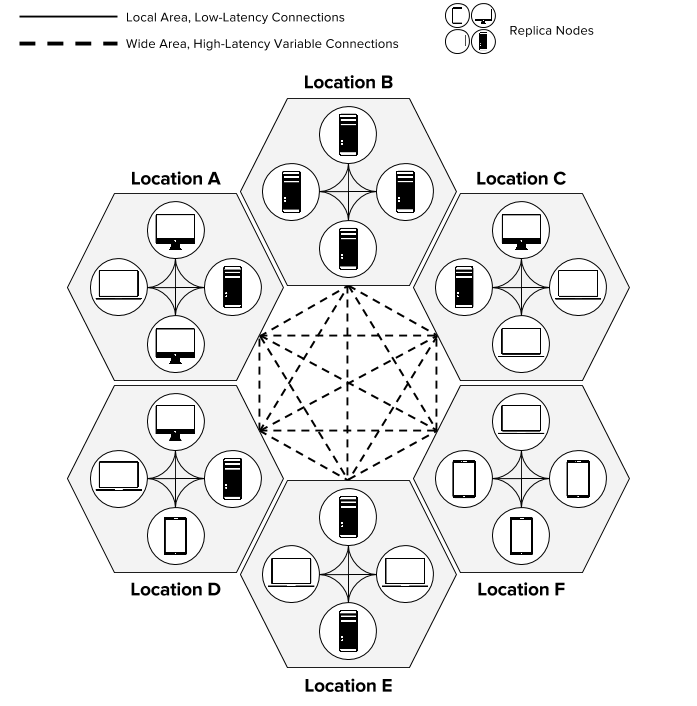
\includegraphics[width=0.5\textwidth]{figures/topology}
    \caption{A topology with many heterogenous replicas operating in a variable latency, partition and failure-prone environment.}
    \label{fig:topology}
\end{figure}

In order to investigate the effect of variable latency and the network environment on consistency, we have constructed a fully connected topology of replica nodes that are each assigned a geographic region as shown in Figure \ref{fig:topology}. Within each region, replica nodes enjoy stable, low-latency connections with their neighbors. However, across regions the latency is higher and the connections variable, meaning that out of order messages are more common across the wide area than in the local area.

In this type of topology there are two types of failure: node failure and network partitions. \textit{Node failure} occurs when a single node is shut off or stops responding to messages. \textit{Network partitions} occur when it is not possible for messages to be sent or received from a single geographic region. In both cases, two conditions must be dealt with by the replication protocol in order to satisfy correctness criteria: first the fact that accesses may continue at a partitioned node which are not being replicated by the system and second that the partitioned nodes are behind the global state and must be brought up to date.

\subsection{Logs and Accesses}

Because consistency is defined in terms of an ordering of operations that change the state of a replica, each node maintains a log of operations whose ordering and staleness can be reasoned upon. The question then becomes what those operations are in the context of a file system. A first attempt might be to map all reads and writes as individual operations that must be ordered, however that would be inefficient if the accesses are at the level of buffered system reads and writes. Instead, distributed systems usually aggregate individual accesses into \textit{Close-To-Open} (CTO) consistency where read and write accesses are ``whole file'' \cite{muthitacharoen_low-bandwidth_2001}. Furthermore, with respect to local accesses we guarantee that a read returns the last write (given no remote updates, \textit{Read Your Writes Consistency}\pjk{cite}) and that writes are atomic with respect to each other (\textit{Monotonic Write Consistency}) \cite{bermbach_consistency_2013}.

\note{Both Read your Writes and Monotonic Write consistency are outlined in \cite{terry_session_1994,bermbach_consistency_2013,vogels_eventually_2009} with no references; I can report all three above at the end of the sentence?}

Each replica's log therefore is composed of a series of write accesses to multiple objects. Each object has a unique name that identifies it to the system and a monotonically increasing version number which can be implemented either as a vector clock \cite{parker_detection_1983} (or a simple Lamport scaler) in the case of a fixed topology or as a vector stamp \cite{almeida_version_2002} in the case of dynamic topologies. Therefore a write access encapsulate the following information: the name of the object being written to, the parent version of the object to which the write is being applied, the versions and object names of any other dependencies, the replica id where the write occurred, , and an array of blob ids that compose the file at the conclusion of the write.

A read access to a particular object simply looks up the latest local version of that object. Because dependency information can be embedded into a write, it is not necessary to include read accesses in the log. For example, in order to create a transaction that reads from objects $X$ and $Y$, performs a computation then updates objects $Y$ and then $Z$: the write to $Y$ would include as a dependency the earlier version of $Y$ and the read version of $X$ and the write to $Z$ would include the updated version of $Y$ and the read version of $X$. Other notions of dependencies include implicit session dependencies, e.g. all writes are dependent on any access that occur within a minimum time threshold of each other, or explicit dependencies that are added by the application.

Because our system model accounts for heterogenous devices and each write in the log is simply metadata about the version of a file we consider version replication as a separate issue from object or blob replication. Furthermore, system consistency depends only on the replication of version information since a version defines what is visible on each replica to be read (and writes follow an implicit read). While a version must become visible (replicated to) all devices in order for the system to be consistent, the blobs that make up data may not be stored on all devices with different storage resources. If a read access requires blobs that it doesn't have, it can simply request them from a local neighbor that does, or from the origin replica itself. For that reason, the rest of this paper will focus on version replication whose primary resource constraint is latency not bandwidth.

\section{Consistency Model}

In the previous section, we fixed the client-centric definition of consistency by guaranteeing that accesses should provide at least \textit{Monotonic Writes Consistency} (MTO), which states that two updates by the same client will be serialized in the order they arrive. Because every write maintains its parent version there is an explicit ordering to how writes must be applied. Additionally clients are guaranteed the less strict \textit{Read Your Writes Consistency} (RYWC) such that any accesses after a write to version $n$ will return a version $\geq n$. These client-centric views of consistency ensure that standard file system semantics apply at a local level, though not necessarily globally \cite{bermbach_consistency_2013}.

Our consistency model is therefore a \textit{data-centric} model which concerns two primary dimensions: ordering and staleness. Given that every replica maintains a local log of accesses with respect to some abstract total ordering based on the sequence of version numbers and potentially concurrent operations, we can define those dimensions as follows:

\begin{enumerate}
    \item \textit{Ordering} refers to how closely individual logs adhere to the abstract global ordering. A \textit{strict ordering} requires every single log to be exactly the same whereas weaker ordering allows some divergence in the order writes are stored in the log.
    \item \textit{Staleness} refers to how far behind the latest global version a local log is and can be either expressed by the visibility latency of replicating a version to all replicas or simply by how many versions the latest is behind by.
\end{enumerate}

Most data-centric consistency models do not consider staleness but instead refer to the strictness of ordering guarantees and the method by which updates are applied to the state of the replica. Indeed, ordering strictness can lead to increased staleness because writes cannot be accepted until they have fulfilled their dependencies first, creating further delay. Our consistency model considers instead the primary symptom of stale reads and writes: \textit{forks}.

\begin{description}
    \item[\textbf{Fork}] A fork occurs when two replicas concurrently write a new version to the same parent object. Forks introduce inconsistency because there are now two potential orderings of updates to the log, but forks are primarily the symptom of staleness; e.g. the second writer wrote to a stale version of the object.
\end{description}

\begin{figure}[t]
    \centering
    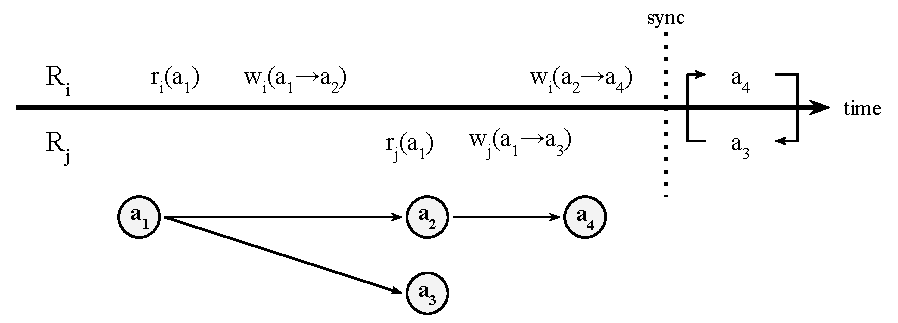
\includegraphics[width=0.5\textwidth]{figures/forks}
    \caption{Accesses before synchronization cause stale reads and forked writes.}
    \label{fig:forks}
\end{figure}

All consistency models discussed in this paper with the exception of \textit{linearizability} are susceptible to forks because they allow stale reads to occur. A fork occurs for a single object when two replicas, $i$ and $j$ read object version $A_1$ and then accesses $W_i(A_1)$ and $W_j(A_1)$ occur creating two new versions, $A_2$ and $A_3$ with the same parent version $A_1$ before synchronization can occur as shown in Figure \ref{fig:forks}. There are two primary causes of forks: concurrent accesses by multiple replicas and stale reads. The former is distinguished from the latter only if the possibility of synchronization could have occurred. From the point of view of the system, they are identical causes. Forks can branch to arbitrary lengths as replicas continue to write to their latest local copies, however when synchronization occurs a decision as to which ordering of writes is correct must occur.

With this context and consistency model in mind, we can now identify several consistency models in order of increasing ordering strictness and define how each model's correctness criteria responds in the face of forks.

\subsection{Weak Consistency}

A weakly consistent system makes no guarantees whatsoever about the relationship of local vs. remote writes and whether or not any given update will become visible \cite{vogels_eventually_2009}. Weak consistency is often described as ``replicas might get lucky and become consistent'' and in fact a weakly consistent implementation may not have a synchronization protocol whatsoever \cite{bermbach_consistency_2013}.

Weakly consistent systems may have a role in a Federated environment, however. Consider a simple weak consistency synchronization protocol where any remote updates are accepted so long as they do not conflict with any local updates. This model may be used in the case of a replica that expects to be intermittently offline or unable to perform any conflict resolution. By accepting non-conflicting updates the replica can keep up as much as possible with the rest of the system while protecting a core set of objects that the device will routinely access. For example, in mobile mesh sensor networks, each sensor will be frequently writing to its own objects, updating their state and generally not conflicting with the measurements recorded by other sensors. A weakly consistent system may assists in propagating updates from remote sensors back to a core replica system that implements stronger consistency.

\subsection{Eventual Consistency}

Eventual consistency is primarily concerned with the final state of all logs in the system given some period of quiescence that allows the system to converge. In this case, all replicas, no matter their log ordering, should have identical final versions for all objects in the namespace. This suggests that eventual consistency requires some \textit{anti-entropy} mechanism to propagate writes and a policy to handle convergence \cite{terry_managing_1995}. Eventual consistency is very popular for NoSQL databases and hosted distributed storage services \cite{decandia_dynamo:_2007,lakshman_cassandra:_2010} because it favors an optimistic approach to consistency: in most systems conflicts are rare, and if something does go wrong, conflict resolution is up to the application layer. In practice, most applications can handle some inconsistency and moreover the small inconsistency windows due to low latencies in cloud data centers make such conflicts rare and short-lived enough to be worth the risk \cite{bailis_quantifying_2014}.

Eventual consistency implemented by a \textit{last writer wins} policy simply accepts all writes so long as they are more recent than the latest local versions. Eventual reads and writes are always performed locally, and therefore with little performance overhead. Eventual allows forks to occur and moreover allows individual replica logs to have wholly different orderings so long as the last version for each object is in the same given no writes for a long enough period of time. As a result, the latest version of an object may alternate between writes to competing forks (a fairly weak semantic) and in this case, it is up to the application to detect the inconsistency. However, Eventual logs do have one important property - for each object, every write in the log is ordered in a monotonically increasing fashion.

\subsection{Causal Consistency}

Causal consistency provides the strictest ordering guarantee without requiring coordination or consensus \cite{ladin_providing_1992}. In causal consistency all writes that have causal relationships must have those dependencies satisfied, e.g. inserted into the log before that write can become visible. Therefore, even though a write might have been propagated to another replica server it cannot be read until all of its dependencies have also been propagated. Causal consistency can increase staleness particularly when implicit or potential causality creates large dependency graphs that must be resolved before writes can be applied \cite{lloyd_dont_2011}. This can be managed by allowing the application to explicitly specify the dependencies for each write \cite{bailis_potential_2012}.

Our consistency model provides for causality by ensuring that dependencies are tracked along with specific writes to specific versions of objects; in fact every write has at least one dependency, the parent version of the write. Eventual consistency however does not require that the parent version be appended to the log before the write can be made visible, a requirement for causal. Moreover, parent versions only track causality for a single object and do not consider potential causality or ordering of writes to all objects in the namespace. As a result, in order to maintain inter-object causality each write must explicitly specify its dependencies.

\subsection{Sequential Consistency}

Sequential consistency is a strong consistency model that requires that all replicas have the exact same ordering of their logs, such that all writes by all clients are appended in the same exact order \cite{attiya_sequential_1994}. Sequential consistency is not strict in that it does not make guarantees about staleness (or the ordering of reads) but does require that all writes become visible in the same order \cite{bermbach_consistency_2013}. Sequentially consistency is typically implemented with consensus algorithms such as Paxos \cite{lamport_fast_2006} or Raft \cite{ongaro_search_2014} that coordinate logs by defining a transitive, global ordering for all conflicts. Alternatively, sequential consistency and can be implemented with warranties -- time based assertions about a group of objects that must be met on all replicas before the assertions expired \cite{liu_warranties_2014}.

Because sequential consistency allows stale reads to occur forks are still possible, however only a single branch of a forked write can be allowed in the log. Preventing forks would require either a locking mechanism or an optimistic approach that allowed operations to occur but reject all but one branch. Rejecting writes simply passes the buck back to the application that must deal with dropped writes by either retrying or resolving conflicts and writing a new version.

\subsection{Linearizability}

Linearizability is the strongest form of consistency; not only must all write operations occur in sequence, but all operations including reads must be ordered chronologically \cite{herlihy_linearizability:_1990}. A consensus algorithm alone cannot implement linearizability and instead some distributed locking mechanism is required. For example a consensus algorithm can be adapted to instead of making decisions about the total ordering of conflicting writes, granting or releasing locks from requestors, however this opens up the potential for deadlock and extremely poor performance, defeating the purposes of replication in the first place! Data center environments that don't have to deal with issues of clock skew by using super precise atomic and GPS clocks can use precise time measurements to enable a distributed two phase commit protocol \cite{corbett_spanner:_2013}, however every replica is required to have such a time piece, which is not practical for heterogenous topologies.

\section{Federated Consistency}

The Federated Consistency model allows individual replicas to select their own local consistency policies and engage in replication according to the mechanism specified by the policy. Each replica maintains its own local state which is modified in response to local accesses as well as the receipt of messages from remote replicas. Each replica sends messages to other nodes in order to propagate the latest writes as well as to perform housekeeping. Therefore every replica can be seen as an event handler that responds to local access events as well as remote messages and generates more events (sent messages) in return. Simply put, so long as every federated replica has an event handler for all types of RPC messages, federation only has to be defined at the \textit{consistency boundaries}, that is when replicas of one consistency type send messages to that of another.

Given the consistency models discussed in the previous section, we will omit weak consistency as being too simplistic and linearizability as being too performance restrictive. Instead we will focus on the federation of eventual consistency, implemented with latest-writer wins gossip based anti-entropy, and sequential consistency implemented with the Raft consensus algorithm.

\subsection{Gossip-Based Anti-Entropy}

Eventual consistency is implemented by periodic \textit{anti-entropy} sessions that converge replicas towards the same state (e.g. reducing entropy, the divergence between the states of individual replicas) \cite{kempe_gossip-based_2003}. On a routine interval, specified by the \texttt{anti-entropy delay} timing parameter, a replica will randomly select one of the other replicas in the system and send a \texttt{Gossip} message that contains the latest version of all objects in the replica's local log. On receipt of the \texttt{Gossip} message, the remote replica will compare the RPC object versions with those in its local log. If the RPC versions are later, it will append the later versions of the object to the log (\textit{last-writer wins}). However if the remote object version is later it will send that version back to the originating node in a \texttt{GossipResponse} message. As a result, our anti-entropy implementation is \textit{bilateral}.

Replicas that implement eventual consistency read locally and write to their local latest version introducing zero read and write latency. Forks are caused by staleness due to the amount of time it takes to propagate a write to the rest of the system, the visibility latency. Visibility latency in this system can be modeled as:

\begin{equation}
t_{visibility} \approx \frac{T}{4} \log_3N + \epsilon
\end{equation}
\pjk{Where does this come from?}
\note{See email -- I came up with this for bilateral anti-entropy}

Where $\frac{T}{4}$ is the \texttt{anti-entropy delay} as computed from the network environment via the tick parameter, $T$, and $N$ is the number of nodes in the system. The epsilon parameter specifies the amount of added latency injected by imperfect gossip neighbor selections, if $\epsilon = 0$ it would mean that on every anti-entropy session, each node perfectly selected another that didn't have the write being propagated; this is an unlikely scenario in a system that selects neighbors based on uniform random probabilities.

\subsection{Raft Consensus}

Sequential consistency is implemented via the Raft consensus algorithm \cite{ongaro_search_2014}. However, consensus alone does not ensure that sequential consistency is implemented and a number of policy decisions about how Raft followers read and write and interact with the leader must be discussed. First, we will present a brief sketch of the Raft consensus algorithm.

All Raft nodes can be in one of three states: \texttt{FOLLOWER}, \texttt{CANDIDATE}, and \texttt{LEADER} and all replicas are initialized in the \texttt{FOLLOWER} state. Raft is governed by two primary timing parameters: the \texttt{heartbeat interval}, which specifies how often the leader sends \texttt{AppendEntries} messages that double as term keep-alive messages, and the \texttt{election timeout}, an interval in which a uniform random delay is chosen if by which a follower doesn't hear from the leader, it will convert to a candidate and attempt to gain enough votes to become a leader. After initialization, one of the replicas will timeout waiting for an \texttt{AppendEntires} and will send \texttt{VoteRequest} messages with a monotonically increasing term id. Replicas will vote for the candidate if and only if the term is greater than their term and if they haven't voted for anyone in the current term. Once a candidate receives a majority of votes from other replicas it becomes the leader.

The Raft leader has the primary responsibility of coordinating all other Raft replicas. To that end, the leader will broadcast periodic \texttt{AppendEntries} messages to all other Raft followers in order to maintain their leadership for the given term. A write access that originates at a follower must be sent as a \texttt{RemoteWrite} to the leader. The leader accepts writes in the order that they are received, and if the leader detects a fork -- that is that a write has a parent version who already has a child version in the log -- Raft will simply reject (drop) the write. In order to minimize the number of messages that Raft sends, Raft will aggregate all writes into the next \texttt{AppendEntries} message and send them together.

Because all writes that originate at followers are forwarded to the leader, the leader can guarantee a sequential ordering of updates. Therefore on receipt of an \texttt{AppendEntries} message, followers simply add the entries to their log and respond with their last index. If a majority of followers append entries to their logs, the leader will mark those entries as committed and inform the followers the write has been committed on the next \texttt{AppendEntries}.

However, although all writes are sequentially ordered, Raft nodes must decide what to do read, and there are several options:

\begin{enumerate}
    \item \textit{READ COMMITTED} Raft replicas will only read the latest committed version of an object, guaranteeing that the write will not be rolled back in the case of an outage. However, this read mode introduces the potential for a lot of staleness and therefore forks.
    \item \textit{READ LATEST} Raft replicas will read the latest version of the object in their log, even if it hasn't been committed. Moreover, replicas will read their own local writes rather than waiting for an \texttt{AppendEntries} to return their write.
    \item \textit{REMOTE READ} Rather than read locally, simply request the latest version from the leader. This introduces the potential for additional latency, but may be faster if the expected message latency is less than the heartbeat interval.
\end{enumerate}

Each of these options has critical implications for the likelihood of stale reads and writes in the system. Replicas would choose read committed if the network was highly partition prone and messages from the leader were unstable and prone to being rolled back. Remote read servers replicas well when the average message latency is far lower than the heartbeat interval, though this could be improved by making the heartbeat interval similar to the network latency. For this reason, we have selected read latest as the most likely scenario for a file system implementing sequential consistency with Raft.

\subsection{Timing Parameters}

Both the eventual and sequential consistency models are hugely dependent on the timing parameters for consistency. In order to select an \texttt{anti-entropy delay}, \texttt{heartbeat interval}, and \texttt{election timeout} we must find some method of relating the timing to the base latency of our system. To do this we introduce a ``tick'' parameter, $T$, that is computed by the observed message latency in the system specified as normally distributed with a mean, $\lambda_{\mu}$ and standard deviation, $\lambda_{\sigma}$. There are two formulations of T: a conservative formulation that is big enough to withstand most variability, and an optimistic formulation that is much faster but will send many out of order messages that can disrupt consistency if there is variability.

\begin{equation}
    T_{conservative} = 6(\lambda_{\mu} + 4\lambda_{\sigma})
\end{equation}

\begin{equation}
    T_{optimistic} = 2(\lambda_{\mu} + 4\lambda_{\sigma})
\end{equation}

Note that both $T_{conservative}$ and $T_{optimistic}$ are variations on other known models. Ongaro and Ousterhout proposes a more conservative $T$ parameter of $10\lambda_{\mu}$ \cite{ongaro_search_2014}, which while correct has very poor performance relative to the access stream. Howard et. al proposes a similar optimistic $T$ parameter, $\lambda_{\mu} + 2\lambda_{\sigma}$ \cite{howard_raft_2015} -- but this does not capture enough of the variability in the networks we propose and leads to out of order \texttt{AppendEntries} messages, which in turn leads to message thrashing and can impair Raft by causing the log to be entirely replayed.

With the $T$ parameter, all timing parameters for all consistency models can be specified in relationship with each other. For example, in order to ensure that eventual and sequential replicas send approximately the same number of messages (e.g. fixing the message budget in resource constrained environments) the timing parameters are as follows:

\begin{itemize}
    \item \texttt{anti-entropy delay} $= \frac{T}{4}$
    \item \texttt{heartbeat interval} $= \frac{T}{2}$
    \item \texttt{election timeout} $= U(T, 2T)$
\end{itemize}

Moreover, $T$ can be adapted at runtime. For eventual nodes, $T$ can be continually updated with respect to observed message latencies. For Raft nodes, the leader can observe message latencies in response to \texttt{AppendEntries} messages and initiate joint consensus in order to change the configuration. Once joint consensus is achieved the new $T$ tick parameter can be applied.

\subsection{Protocol Federation}

\note{Write a description of how federation is implemented and the "silver bullet" to coordinate between eventual and Raft. The following section is excerpted from the proposal.}

A key requirement of Federated Consistency is the opportunity to create heterogeneous systems with no performance cost, e.g. a homogenous eventual cloud and a homogenous Raft cloud will continue to perform equivalently whether or not they participate in a federated cloud. However, we posit that an eventual cloud should benefit in lowered data staleness and in fork frequency from being connected to a strong, central consensus group. Similarly, Raft nodes should be able to use anti-entropy mechanisms to replicate data and continue writing even if the leader is unavailable and no consensus can be reached to elect a leader. The question is therefore how to integrate the eventual consistency via gossip and sequential consistency via consensus in a non-invasive way.

The central problem is that eventual and Raft clouds choose the ``winner'' of a fork in exactly opposite ways. Eventual clouds choose the last of a set of conflicting writes through a latest-writer wins policy, whereas Raft clouds effectively choose the first by dropping any write that conflicts with any previously seen writes. Our insight is that if the strong central quorum can somehow make an accepted version ``more recent'' than a dropped fork, then the propagation of the fork would cease in the eventual cloud, reducing the possibility of continued forks.

In order to federated multiple consistency models, there are two integration points: communication and consistency. Our initial approach was to integrate communication at the Raft nodes, by allowing Raft nodes to participate in anti-entropy with the eventual cloud (but not other Raft nodes). Eventual nodes therefore ``synchronize'' with a local Raft node (modified by some synchronization probability) by exchanging \texttt{Gossip} messages with the Raft nodes. A slight increase in the synchronization probability balanced the amount of synchronization with the amount of communication in the eventual cloud given the imbalance in the ratio of eventual nodes to Raft nodes. In order to manage the communications delay between the anti-entropy timeout and leadership coordination, Raft nodes must keep local caches of forked or dropped writes so as to not propagate them back to the eventual cloud or replay them to the leader. However, we have observed that this was not enough to stop the eventual cloud from propagating a fork around Raft, causing further inconsistencies.

Our approach to integrate consistency is to extend each version number with an additional monotonically increasing counter called the \textit{forte} (strong) version that can only be incremented by the leader of the Raft quorum. Because the Raft leader dropped forks or any version that was not more recent than the latest version, incrementing the forte number on commit ensures that only consistent versions are marked. In order to determine the latest version, the forte number is compared first, then the version number, allowing Raft to ``bump'' the consistent version to a more recent version. In order to prevent that version's children from becoming less recent, on receipt of a version with a higher forte than the local, eventual nodes must search for the forte entry in their local log, find all children of the update, and set the child version's forte equal to that of the parent.

Our preliminary investigations show that this integration works well to curb inconsistencies due to anti-entropy delays as well as those introduced by communication integration. There are, however, quite a few knobs to turn in the system described above. Further investigation into smoothing integration points between consistency protocols and the policies that each define may lead to smoother messaging with fewer resource constraints. We have identified a current bottleneck in the system however: the leadership of the central quorum, through which every single write must pass, no matter the size of the cloud. In order to address this, we propose an adaptation to the central consensus group such that it can provide Hierarchical Consensus.

\section{Simulation Results}

\begin{figure*}
    \centering
    \minipage{0.5\textwidth}
      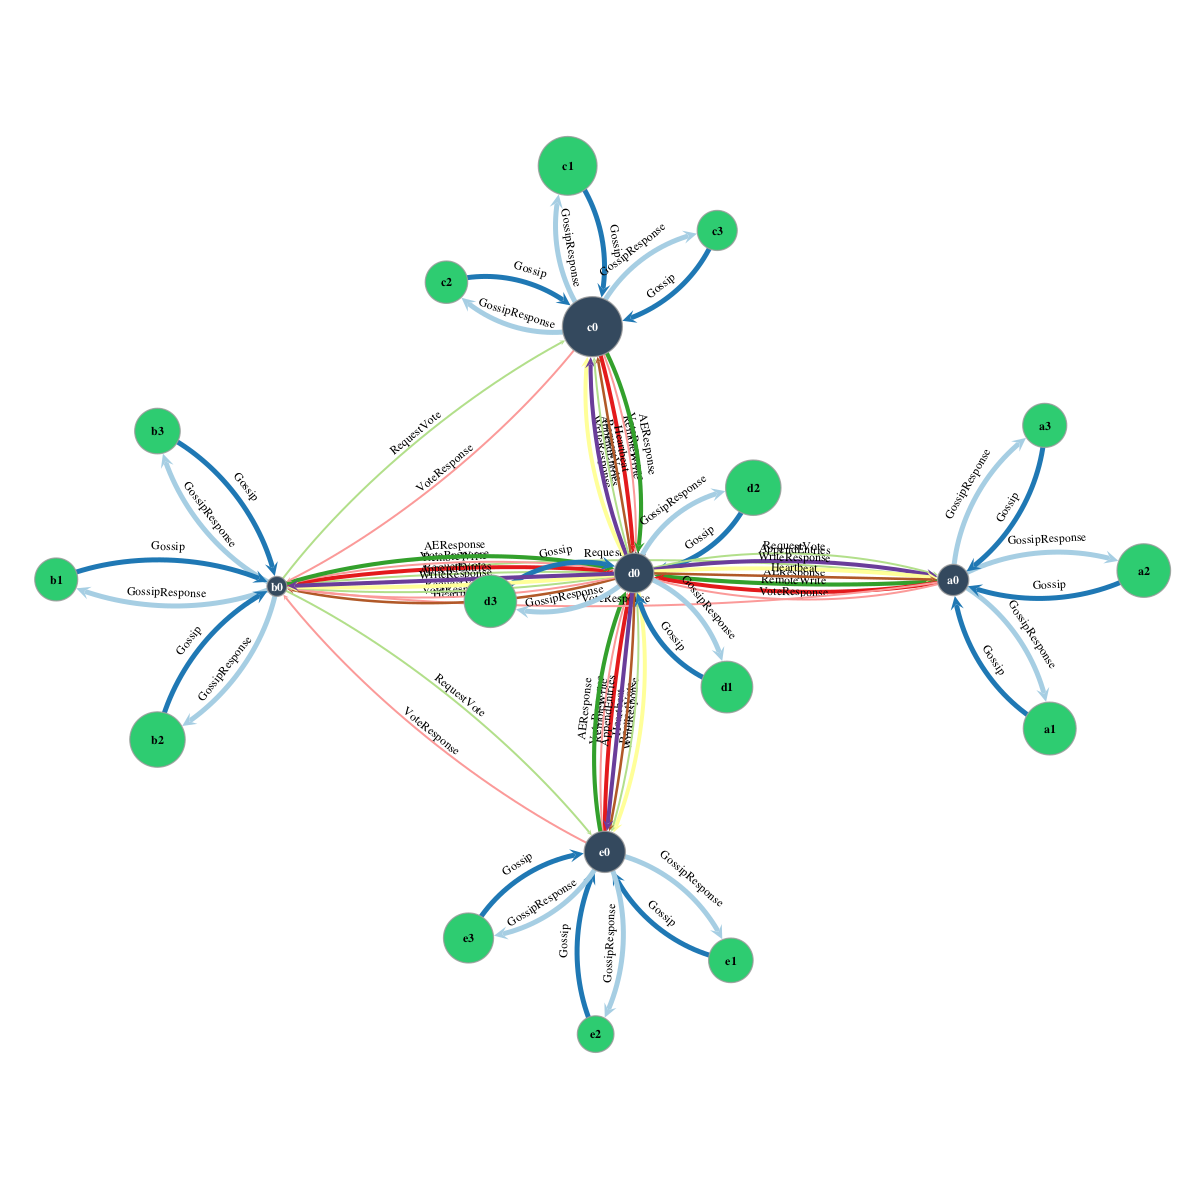
\includegraphics[width=\linewidth]{figures/conflict/federated_sync}
      \caption{Accesses in a Federated topology with primary Raft synchronization.}\label{fig:federated_sync}
    \endminipage\hfill
    \minipage{0.5\textwidth}
      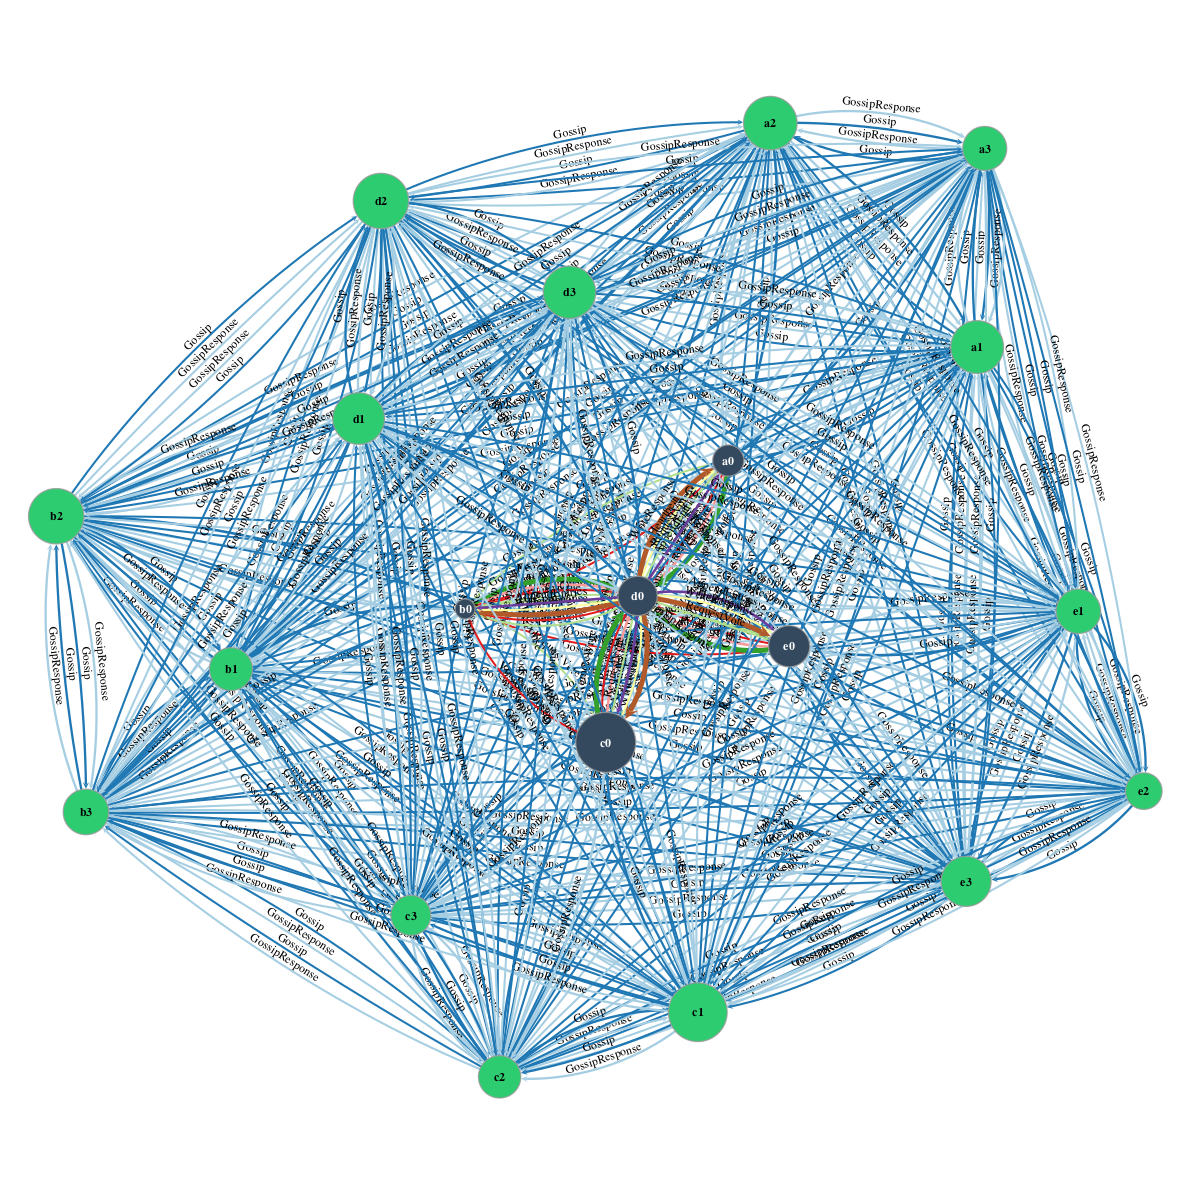
\includegraphics[width=\linewidth]{figures/conflict/federated_eventual}
      \caption{Accesses in a Federated topology with a preference for wide area anti-entropy over synchronization.}\label{fig:federated_eventual}
    \endminipage\hfill
\end{figure*}

In order to evaluate a federated model of replication and consistency, we have created a discrete event network simulation that allows us to flexibly configure a variety of parameters and more closely investigate the behavior of replication. The input to the simulation has two parts: a topology that specifies the replicas and network environment; and a workload of access events to named objects. The simulation instantiates each replica as a process that executes read and write accesses to objects and generates replication messages as well as listens for and handles messages from other replica servers.

Each topology specifies each device as an independent replica server, by uniquely identifying it with device-specific configurations. By far the most important configuration is the \textit{replica consistency} (or replica protocol) which determines the replica's behavior in the environment. For the purposes of our simulation we have proposed three types of eventual and sequential consistency implementations:

\begin{itemize}
    \item \textbf{Eventual}: Eventual nodes perform replication via anti-entropy by random selection of a neighbor to do pairwise gossip with. Eventual nodes can prioritize local vs. wide area nodes by specifying $P_{local}$ -- the likelihood of local neighbor selection.
    \item \textbf{Stentor}: A ``Stentor'' node is an eventual node that performs \textit{two} anti-entropy sessions per interval, always choosing one local and one remote node. We have implemented Stentor nodes to show that Raft isn't simply acting as a minimum spanning tree in the network, but is also preserving consistency guarantees.
    \item \textbf{Raft}: Raft nodes implement the Raft consensus protocol, electing a leader and forwarding writes to the leader to maintain a sequential ordering. If a write is forked, the leader will drop it in order to maintain our consistency guarantee.
\end{itemize}

The topology further specifies the \textit{location} of each device, the \textit{connections} between devices, and the \textit{distribution} of message latency on a per-connection basis. There were two primary latencies specified as normal distributions ($\lambda_{\mu}$, $\lambda_{\sigma}$), the \textit{local area} latency, usually with a lower $\lambda_{\mu}$ and $\lambda_{\sigma}$ than the \textit{wide area} latency -- e.g. the latency between devices in different locations. In order to compute the tick parameter, $T$, and specify the average latency in the simulation, latencies are given as the worst case, wide-area latencies. Each topology could also set simulation-specific configurations, as well as device-specific configurations.

The workload was specified as access trace files -- time ordered access events (reads and writes) between a specific device and a specific object name. Each trace was constructed via a random workload generator, where a collection of available devices was specified along with a normal distribution of the delay between accesses ($A_{\mu}$, $A_{\sigma}$), the number of objects, $o$, in the system, and a probability of conflict, $P_c$. To generate the workload, object names were assigned to each replica as follows: in a round-robin fashion, an object name was selected and assigned to a replica with probability $P_c$ until each replica was accessing $o$ objects. If $P_c = 1.0$ then every single replica would be accessing the same batch of objects, where as if $P_c = 0.0$ then each replica would access their own unique set of objects. From there, the $A_{\mu}$, $A_{\sigma}$ was used to generate accesses to objects in sequence, by selecting an object and reading and writing to it over time until some probability of switching objects occurred. In effect, the final workload simulates multiple replicas reading and writing at a moderate pace for approximately one hour.

Examples of topologies and accesses are shown in Figures \ref{fig:federated_sync} and \ref{fig:federated_eventual}; these graphs show our primary simulation topology of 20 nodes, 4 nodes each in 5 wide areas, the size of vertices represents the number of accesses that occur at that location and the color represents the replica type, the edges are colored by RPC type and sized by the number of messages. These figures show that minor changes in the topological configuration can lead to dramatic changes in the message traffic in the system; both of these figures show a federated topology of a small Raft core group surrounded by eventual clients however Figure \ref{fig:federated_eventual} has a preference for anti-entropy across the wide area whereas Figure \ref{fig:federated_sync} has a preference to synchronizing with the local Raft node.

\subsection{Experiments and Metrics}

We conducted two primary experiments to test the behavior of a federated consistency system against homogenous Raft and homogenous Eventual systems. The first was to test the behavior of increasing conflict, $P_c$ and the second was to explore the effect of the network environment in terms of the mean latency, $\lambda{\mu}$ of the wide area. The input to the system was a fixed topology of 20 nodes in 5 wide areas, along with an access trace that contained approximately 29,000 accesses (depending on the experiment), with an average ratio of 54\% of the accesses being reads \pjk{Why 54\%? More generally you need to motivate our choices for trace and topology.}.

Our primary metrics are \textit{forked writes} and \textit{stale reads}. We define forked writes as the number of writes that had more than one child, whereas a read is stale if it returns anything other than the globally latest version. A further metric of \textit{inconsistent writes} measured the number of writes whose parent was forked allowed into the log of a replica, as balanced by the number of \textit{dropped writes} --- writes that the sequential ordering Raft nodes would reject as being invalid.\pjk{Motivate all.}

Furthermore the cost of each replication protocol was measured in terms of the number of \textit{sent messages} as well as latencies of various RPC calls. Some latencies were dependent if the protocol specified \textit{cached} or \textit{remote} accesses: the \textit{read latency} and \textit{write latency} measured the amount of time an access took until a response was returned to the client. In the case of Eventual nodes, this latency was zero, since an eventual node always responds with cached information; however Raft required remote accesses to the leader in order to respond. Other latencies were global, e.g. the \textit{visibility latency} specifies the average amount of time it takes a write to become fully visible, that is replicated to all nodes in the network. Any writes that do not become fully visible (stomped on through the eventually consistent policy of latest writer wins) are ignored. This metric is closely related to the \textit{percent visible} metric --- the average number of replicas a write is propagated to. Finally the \textit{commit latency} specified how much time was required for a write to be committed, e.g. confirmed as accepted by a quorum of nodes.

\subsection{Conflict Probability}

\begin{figure*}
    \centering
    \minipage{0.32\textwidth}
      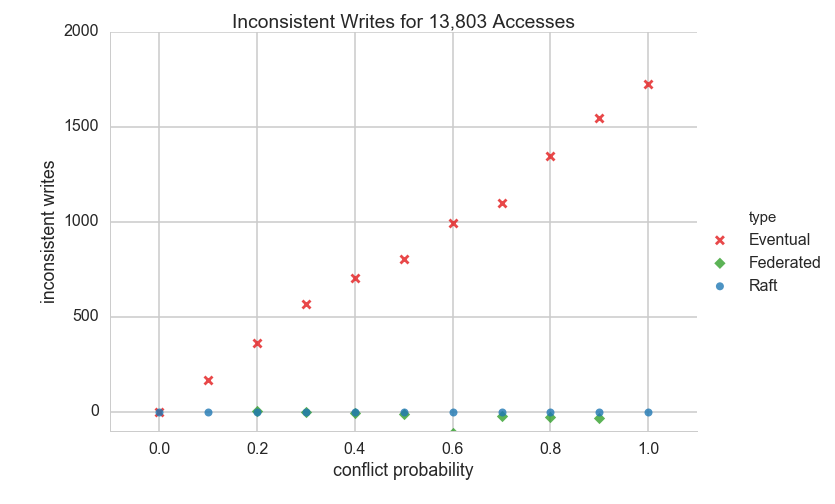
\includegraphics[width=\linewidth]{figures/conflict/inconsistent_writes}
      \caption{Inconsistent writes by increasing conflict.}\label{fig:inconsistent_writes}
    \endminipage\hfill
    \minipage{0.32\textwidth}
      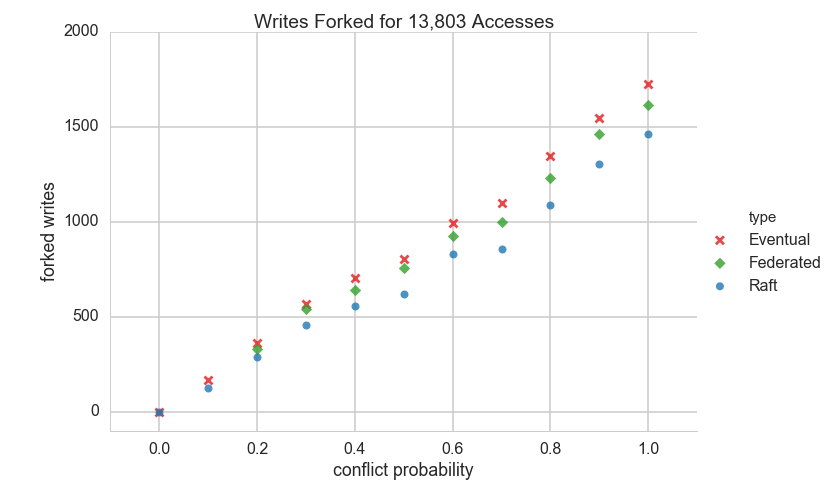
\includegraphics[width=\linewidth]{figures/conflict/forked_writes}
      \caption{Forked writes caused by increasing conflict.}\label{fig:forked_writes}
    \endminipage\hfill
    \minipage{0.32\textwidth}%
      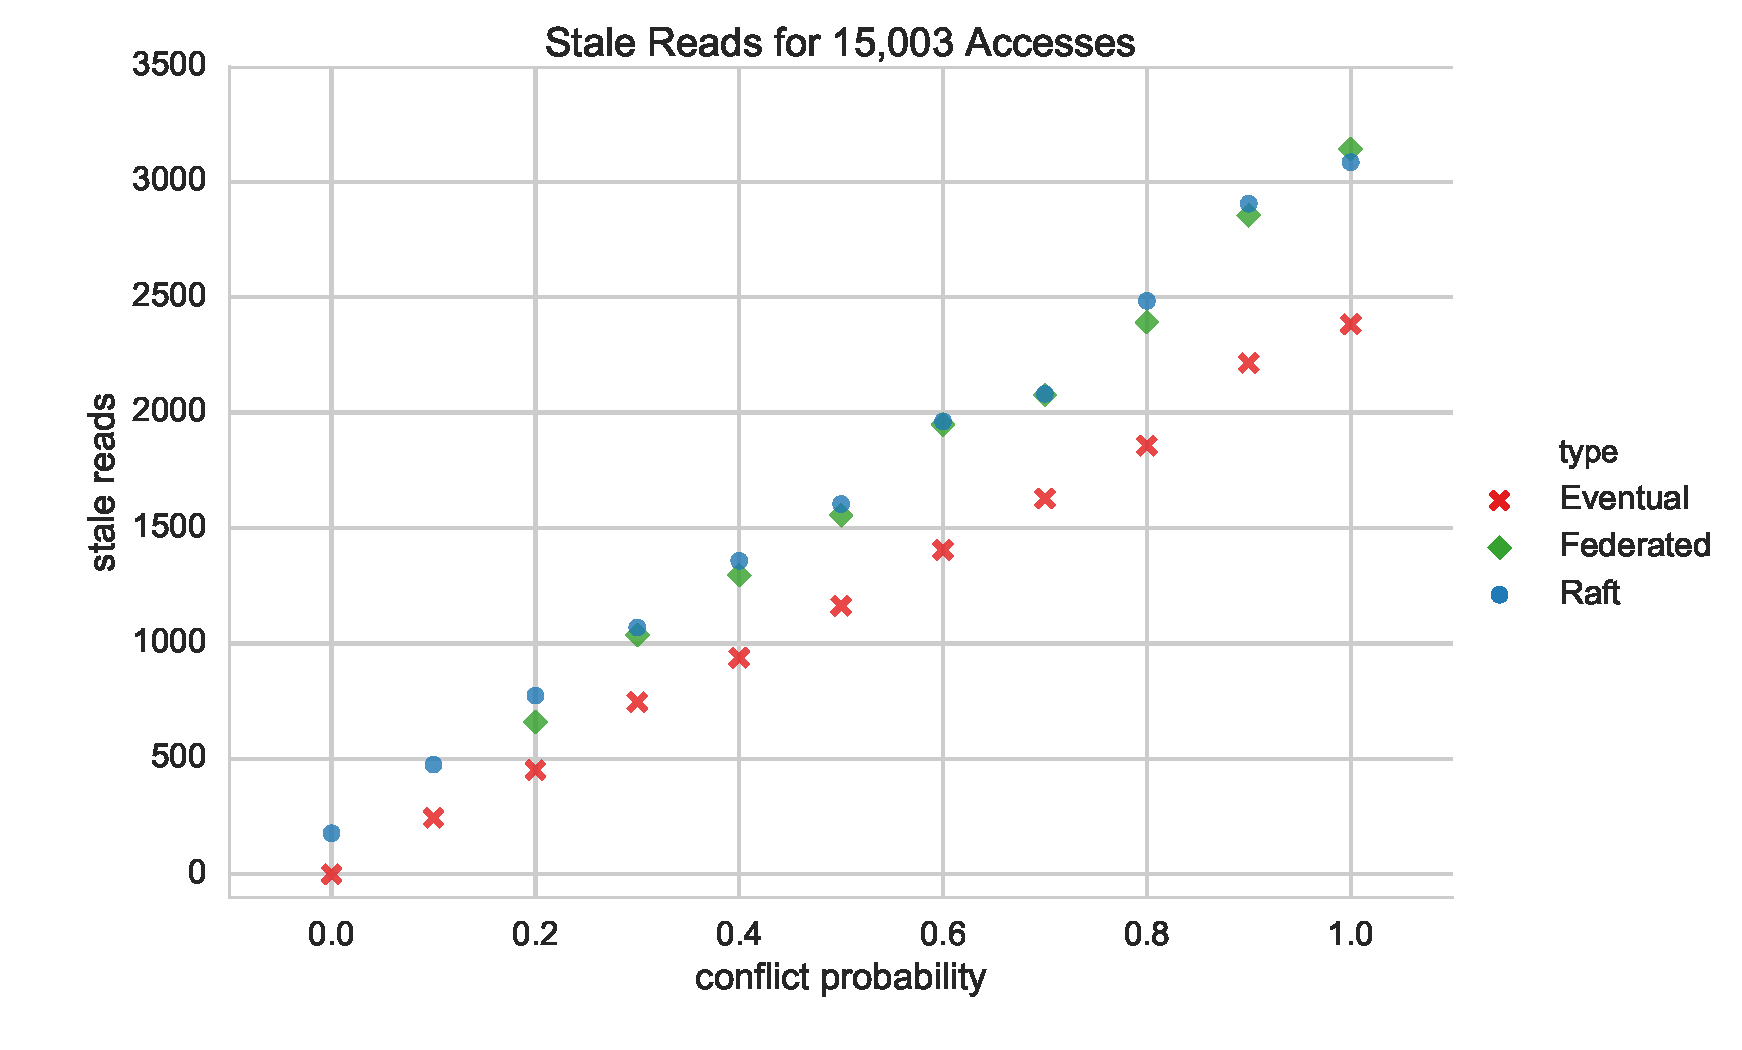
\includegraphics[width=\linewidth]{figures/conflict/stale_reads}
      \caption{Stale reads as conflict increases.}\label{fig:stale_reads}
    \endminipage
\end{figure*}

In this experiment we ran 44 simulations, each of which specified a combination of consistency type: one of \textit{homogenous eventual}, \textit{homogenous raft}, \textit{federated eventual with 5 raft nodes}, and \textit{federated eventual with 5 stentor nodes} as well as a $P_c \in [0.0,1.0]$ with a step of $0.1$. In particular, we wanted to show how a Federated system would behave in the best case scenario for all replication protocols (no conflict, each replica accesses only their own objects) to the point where conflict is guaranteed because all replicas are trying to read and write to the same small set of objects.

As shown in Figure \ref{fig:inconsistent_writes}, as the conflict in the system increases, eventual methodologies suffer from more and more inconsistent writes\pjk{And we care because...}. Eventual nodes do manage forks or ordering of accesses\pjk{huh?}, but simply write to the latest version. This has benefits in that eventual nodes can respond quickly, and in fact as shown in \ref{fig:stale_reads}, eventual systemshave low numbers of stale reads even as conflict increases. However, as shown in \ref{fig:forked_writes}, the inconsistencies that are in the eventual nodes match the number of forked writes in the system\pjk{so?}. However, both Raft and Federated systems eliminate inconsistencies (Federated allows a few in higher conflict scenarios) by simply dropping writes. \pjk{Why is this important? User view of data more orderly?}

\subsection{Latency Variation}

\begin{figure*}
    \centering
    \minipage{0.5\textwidth}
      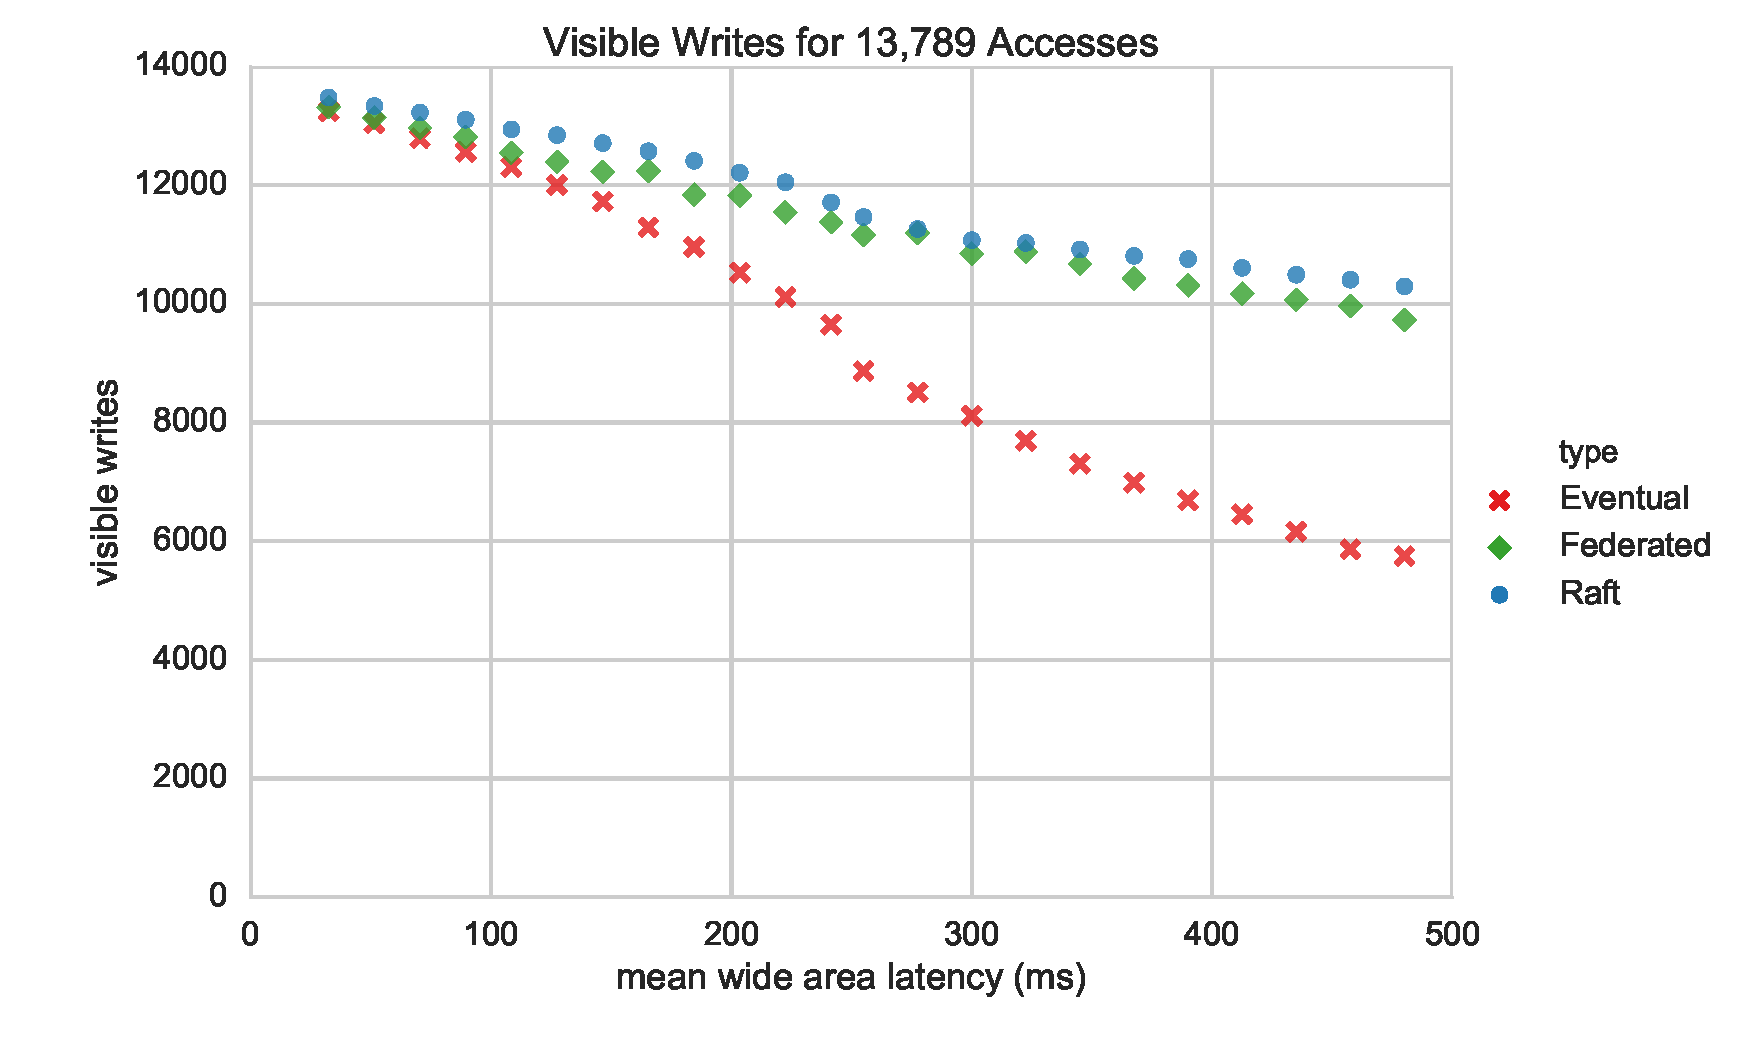
\includegraphics[width=\linewidth]{figures/latency/visible_writes}
      \caption{The percentage of fully visible writes.}\label{fig:visible_writes}
    \endminipage\hfill
    \minipage{0.5\textwidth}
      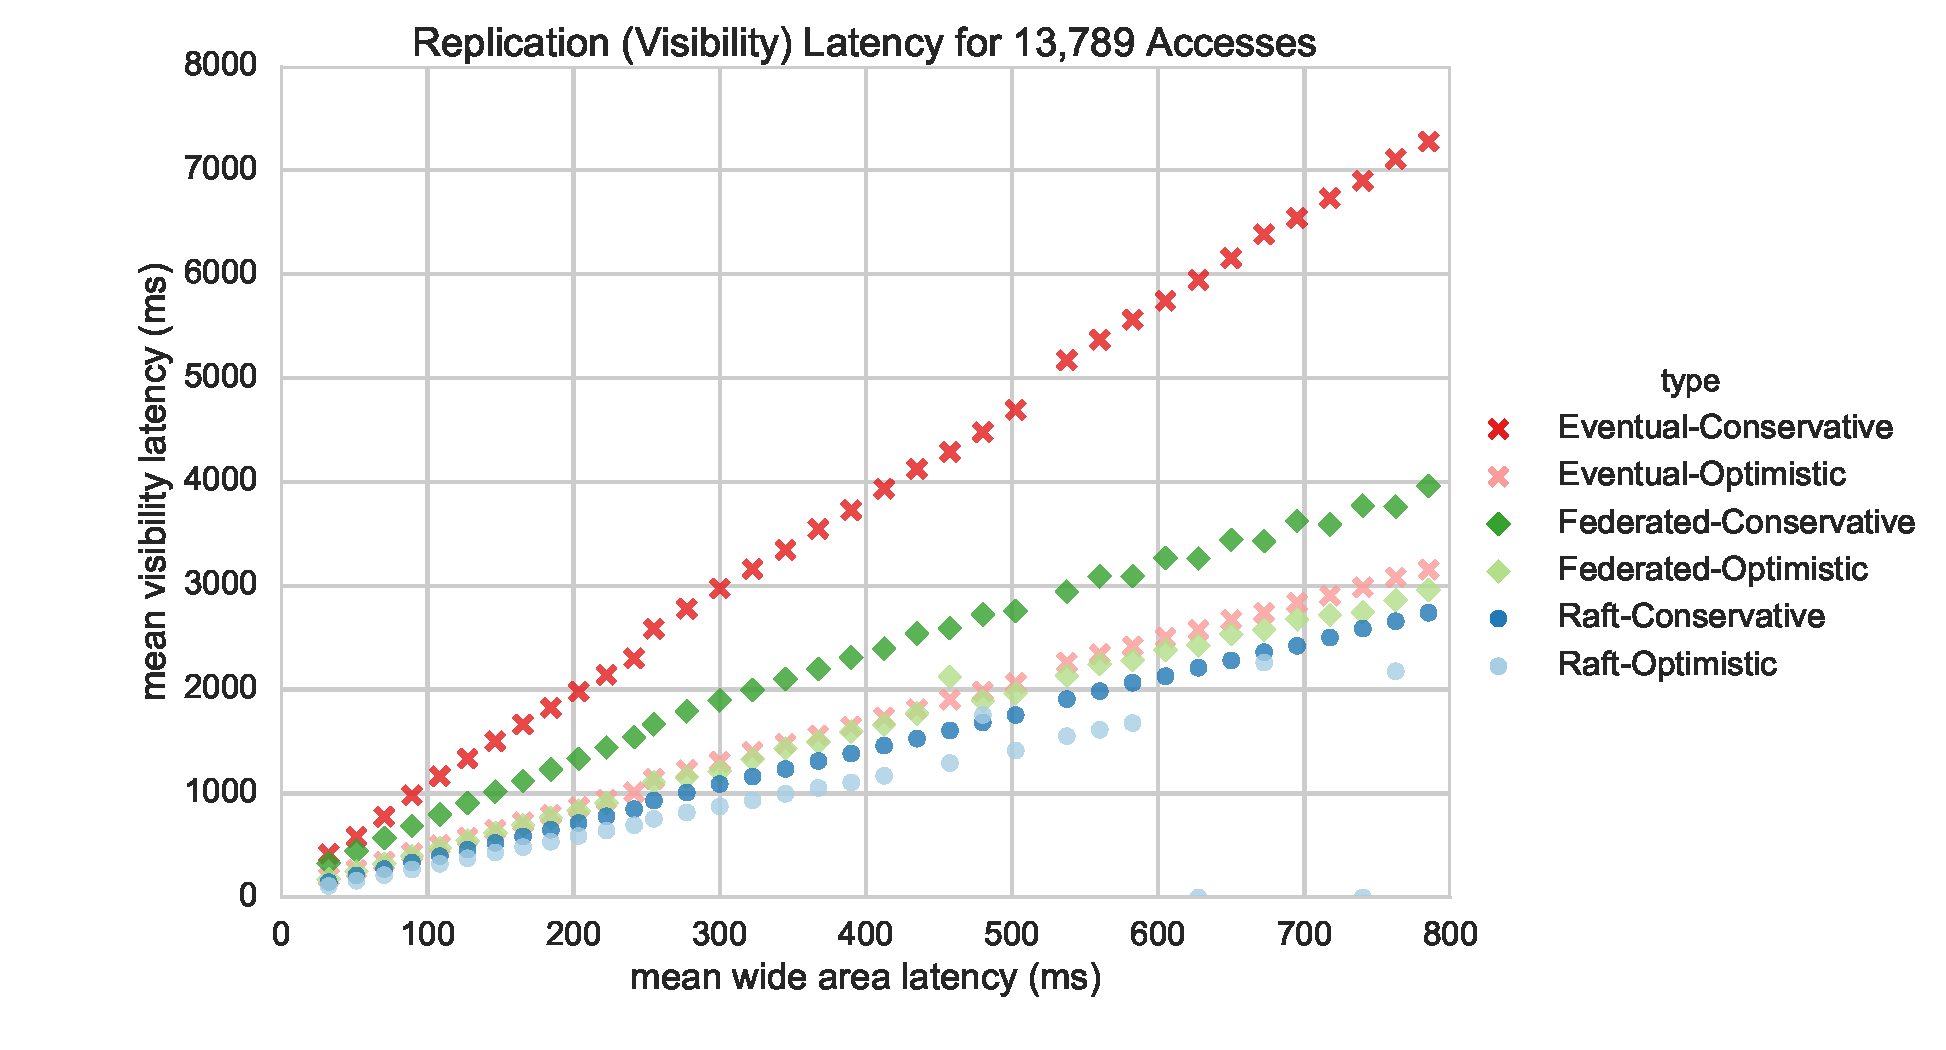
\includegraphics[width=\linewidth]{figures/latency/visibility_latency}
      \caption{The average full visibility latency.}\label{fig:visibility_latency}
    \endminipage\hfill
\end{figure*}

\begin{figure*}
    \centering
    \minipage{0.32\textwidth}
      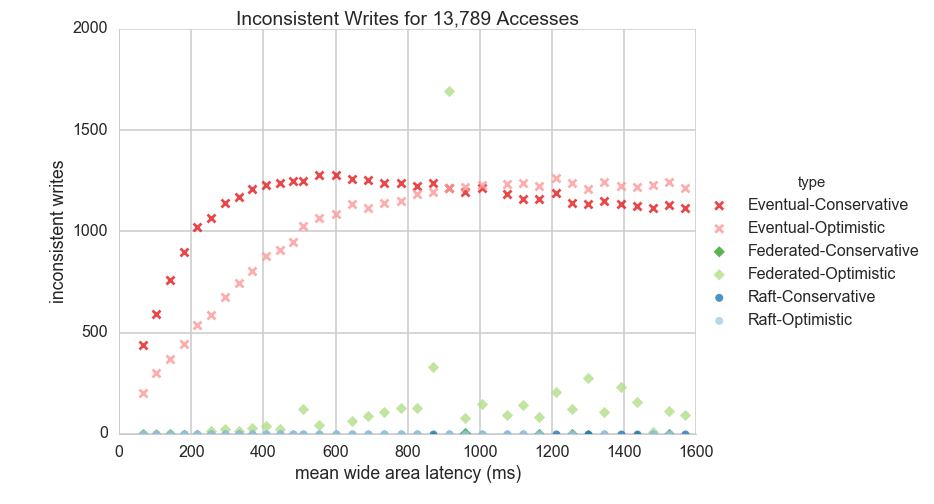
\includegraphics[width=\linewidth]{figures/latency/inconsistent_writes}
      \caption{The number of inconsistent writes written to the log of a replica.}\label{fig:latency_inconsistent_writes}
    \endminipage\hfill
    \minipage{0.32\textwidth}
      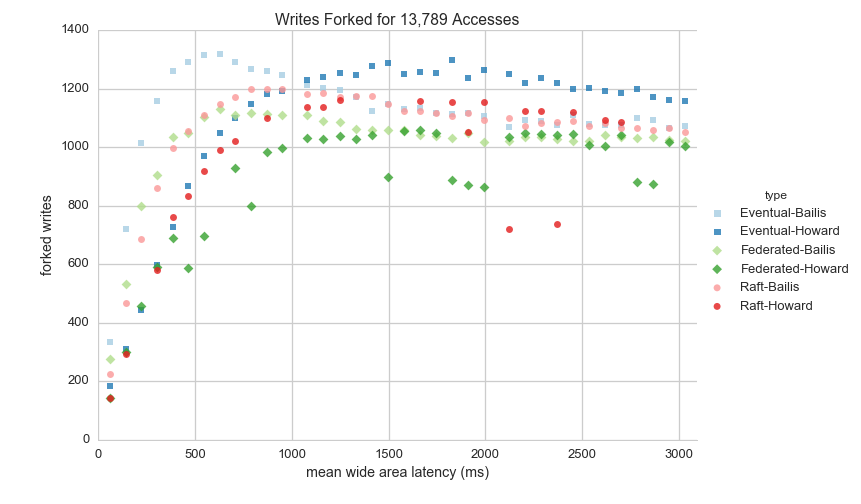
\includegraphics[width=\linewidth]{figures/latency/forked_writes}
      \caption{The total number of conflicts (possible forks).}\label{fig:latency_forked_writes}
    \endminipage\hfill
    \minipage{0.32\textwidth}%
      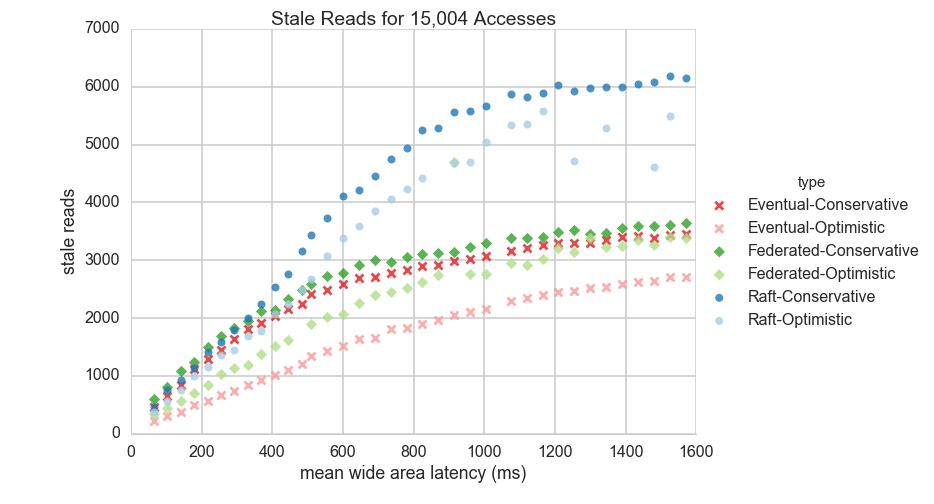
\includegraphics[width=\linewidth]{figures/latency/stale_reads}
      \caption{The percent of reads that are stale in the system.}\label{fig:latency_stale_reads}
    \endminipage
\end{figure*}

In the second experiment we ran 216 experiments to test the effect of variable network latency on consistency protocols as well as on how the selection of the tick parameter model affects consistency for each system. We specified 12 wide area mean latencies in three categories: low ($\lambda{\mu} \in [40,500]ms$ with a low $\lambda_{\sigma}=10.0$), medium ($\lambda{\mu} \in [500,1000]ms$ with a moderate $\lambda_{\sigma}=20.0$), and high ($\lambda{\mu} \in [1000,1500]ms$ with a high $\lambda_{\sigma}=30.0$). In each of these environments we ran three replication models: \textit{homogenous eventual}, \textit{homogenous Raft}, and \textit{federated eventual and Raft}.

Each of these 108 simulations was then parameterized with two different $T$ parameters, computed by the wide area $\lambda_{\mu}$ and $\lambda_{\sigma}$: $T_{conservative}$ and $T_{optimistic}$. However the access mean, $A_{\mu}$ was fixed at approximately one access per replica every 3000ms. In effect, this meant that for approximately half the simulations (with the higher latencies), it was impossible for a write to become visible on another replica before a fork. Even though we fixed the conflict probability as $P_c=0.5$ there was still enough conflict in the simulation that forced each replica protocol to handle forks.

In terms of consistency metrics, the number of inconsistent writes\pjk{Again, this is a low-level metric that affects other metrics (forks, staleness) that are application/programmer visible. We might want to not even mention IWs except to explain strange results.} is more than halved from eventual in Federated due to the presence of the Raft core (Figure \ref{fig:latency_inconsistent_writes}). This is because Federated can take advantage of the topology where Raft and Eventual cannot - broadcasting across the wide area to minimize the number of pairwise communications in anti-entropy but still allowing available responses with the Eventual core. Similarly, the number of stale reads as shown in Figure \ref{fig:latency_stale_reads} sits between both Raft and Eventual for both the optimistic and conservative tick parameters.

We can characterize this in two ways: first that the propagation is faster in Federated than it is in Eventual, thereby leading to fewer forks. Figure \ref{fig:visibility_latency} shows the average visibility latency, that is the time in milliseconds it takes a version to fully replicate, that is become visible on every node in the network. Raft benefits from a broadcast mechanism, while Eventual must wait for exponential propagation. Federated is somewhat slower than Raft, but outperforms Eventual while still being fault tolerant and highly available. As a result, as shown in Figure~\ref{fig:visible_writes}, the number of fullly visible writes is higher for Federated than Eventual, since there is less stomping on versions (maintained by Raft) and because of the decrease in the visibility latency. Together these two properties give Federated better consistency than Eventual, while still maintaining availability in Raft.
\pjk{I'd say that Fig 11+12 are the core of the paper, and they are quite poor for federated. Please don't forget to get the cumulative staleness numbers.}
\section{Discussion}

A strong central core to provide support to the entire system has been suggested both in Oceanstore \cite{kubiatowicz_oceanstore:_2000} and primary copy schemes \cite{gray_dangers_1996}. We take this idea further in our experiments by Federating a strong central core composed of Replicas that perform consensus via the Raft consensus protocol and combine it with highly available eventually consistent systems. In this way Federated consistency gains the flexibility and availability of the eventual nodes (leader re-election and no requirement for remote writes mean that the node can continue even if it is completely partitioned from the rest of the network) while still getting guarantees from Raft, which minimizes ``fork flipping'' -- the behavior of writing to one branch then another, truly pernicious inconsistent behavior that cannot be prevented in an eventually consistent system.

System designers can take advantage of heterogenous nodes by implementing stronger consistency on more reliable machines that are able to handle more messages. Mobile nodes that are prone to network loss, out of order or missed messages, or other variable behavior can adapt their policy depending on the environment they're in. Our model also allows for \textit{adaptive} behavior, in that the replicas can monitor the environment for change and as the mean latency decreases, adapt their $T$ parameter accordingly. This is a no cost operation for eventual nodes (who can also optimize pairwise gossip by implementing non-discrete random selection using Bandits or other optimization techniques), and only requires joint consensus on the part of the consensus group.

Our simulation implementation gave us the benefit of being able to manipulate many parameters to see how replication behavior changes. As a result, we only focused on the number of consistency messages sent. Potentially this overstates the differences between the protocols; Raft leaders have more processing requirements for example. Additionally bandwidth pressure and differences in messaging might be more important to the overall performance of a system. However, by focusing on the number of messages and isolating version replication from blob replication (e.g. minimizing the amount of data required for consistent behavior), we have allowed each protocol to fix some ``message budget''.

In truly resource constrained environments, allowing both Raft and Eventual (either in a homogenous or Federated context) to maintain an equal or semi-equal message budget by modifying the $T$ parameter and allocating timing similarly means that congestion is reduced or optimized. Moreover, this system also allows for adaptive behavior by providing a single place of modification and optimization; $T$ could be optimized according to a cost function (e.g. the message budget or other real time estimates of performance) or could be boosted for a node that has to do a lot of work. This type of flexibility is important to being able to understand how minor changes in both the environment and protocols effect overall consistency in the system as a whole.

% \pjk{Given bilateral anti-entropy and a large communication budge, nothing beats eventual. In some situations Raft might be ``better'' because it's consensus, but even w/ it we can't implement sequential consistency. So where is raft better?  Everyone sees the current version at the end of an epoch. Note that raft doesn't prevent stale reads, but it does bound the staleness (to the length of an epoch). Eventual doesn't.   W/ federated, we lose the ability to bound staleness tightly, so we need to make sure that we implement out epoch-backpressure. I'm hopeful the resulting numbers will look much better.}

% \note{Since the note above, we've implemented the forte number (backpressure)}

\subsection{Fork Minimization}

The primary form of inconsistency that we are concerned with is a fork, that is two separate, conflicting writes to the same parent version. In a homogenous eventually consistent system implemented with anti-entropy, the only way to minimize the number of forks is by increasing the speed of propagation. We have presented the best case for eventual by implementing \textit{bilateral} anti-entropy as well as neighbor selection likelihoods that lead to exponential convergence of a write. However, with a \textit{latest-writer wins} policy, the possibility of ``branch-flopping'' exists; that is after a fork occurs, the latest version is updated on either side of the branch, and though the system will converge to a final write, branches may be arbitrarily long and represent significantly inconsistent states to the user.

A homogenous Raft system on the other hand simply does not allow forks to occur by requiring that the leader determines which write is accepted and which is not. Because we are aggregating writes in the \texttt{AppendEntries} messages every heartbeat interval, at most $n-1$ forks, where $n$ is the number of nodes, are possible within the heartbeat interval. Whichever remote write arrives at the leader first will be accepted as the canonical branch. Here, the branch length is bounded to the number of writes possible by a single node in the heartbeat interval, which is small -- and the branch is eliminated at the heartbeat interval anyway.

The Federated system must at its core resolve how fork elimination is communicated to the eventual system. A fork, by definition, is later than the earlier version. If the Federated system simply ignores or drops forks, the eventual cloud might still propagate the fork around Raft. Worse, if the eventual portion simply drops forks without deciding on a write to propagate, the system is no longer eventually consistent since it is possible that given no more writes half of the nodes make one fork visible while the other half make the other visible.

\textbf{Note: right now we have Federated simply dropping the fork, which is creating bushier version trees and therefore more dropped writes.}

\section{Related Work}

One of the earliest attempts to hybridize weak and strong consistency was a model for parallel programming on shared memory systems by Agrawal et al \cite{agrawal_mixed_1994}. This model allowed programmers to relax strong consistency in certain contexts with causal memory or pipelined random access in order to improve parallel performance of applications. Per-operation consistency was extended to distributed storage by the RedBlue consistency model of Li et al \cite{li_making_2012}. Here, replication operations are broken down into small, commutative suboperations that are classified as red (must be executed in the same order on all replicas) or blue (execution order can vary from site to site), so long as the dependencies of each suboperation are maintained. The consistency model is therefore global, specified by the red/blue ordering and can be adapted by redefining the ratio of red to blue operations, e.g. all blue operations is an eventually consistent system and all red is sequential.

The next level above per-operation consistency hybridization is called \textit{consistency rationing} wherein individual objects or groups of objects have different consistency levels applied to them to create a global quality of service guarantee. Kraska et al. \cite{kraska_consistency_2009} initially proposed consistency rationing be on a per-transaction basis by classifying objects in three tiers: eventual, adaptable, and linearizable. Objects in the first and last groups were automatically assigned transaction semantics that maintained that level of consistency; however objects assigned the adaptable categorization had their consistency policies switched at runtime based on a cost function that either minimized time or write costs depending on user preference. This allowed consistency in the adaptable tier to be flexible and responsive to usage.

Chihoub et al. extended the idea of consistency rationing and proposed limiting the number of stale reads or the automatic minimization of some consistency cost metric by using reporting and consistency levels already established in existing databases \cite{chihoub_harmony:_2012,chihoub_consistency_2013}. Here multiple consistency levels are being utilized, but only one consistency model is employed at any given time for all objects, relaxing or strengthening depending on observed costs. By utilizing all possible consistency semantics in the database, this model allows a greater spectrum of consistency guarantees that adapt at runtime.

Al-Ekram and Holt \cite{al-ekram_multi-consistency_2010} propose a middleware based scheme to allow multiple consistency models in a single distributed storage system. They identify a similar range of consistency models, but use a middleware layer to forward client requests to an available replica that maintains consistency at the lowest required criteria by the client. However, although their work can be extended to deploying several consistency models in one system, they still expect a homogenous consistency model that can be swapped out on demand as client requirements change. Additionally their view of the ordering of updates of a system is from one versioned state to another and they apply their consistency reasoning to the divergence of a local replica's state version and the global version. Similar to SUNDR, proposed by Li et al. \cite{li_secure_2004}, an inconsistency is a fork in the global ordering of reads and writes (a ``history fork''). Our consistency model instead considers object forks, a more granular level that allows concurrent access to different objects without conflict while still ensuring that no history forks can happen.

Hybridization and adaptation build upon previous work that strictly categorizes different consistency schemes. An alternative approach is to view consistency along a continuous scale with a variety of axes that can be tuned precisely. Yu and Vahdat \cite{yu_design_2002} propose the \textit{conit}, a consistency unit described as a three dimensional vector that describes tolerable deviations from linearizability along staleness, order error, and numeric ordering. Similarly, Afek et al. \cite{afek_quasi-linearizability:_2010} present quasi-linearizable histories which specify a bound on the relative movement of ordered items in a log which make it legally sequential.

\section{Conclusion}

In this paper we have presented a model for federated consistency that allows individual replicas to expose local policies to users while still allowing for global guarantees given a heterogenous system of replicas where at least a core group enforces sequential consistency. By designing a federated system where only the interactions between replicas of varying consistency types are defined, systems can scale beyond the handful of devices usually described to dozens or hundreds of replicas in variable latency, partition-prone geographic networks. As each replica monitors its local environment and the throughput of its communication with other replicas it can adapt as necessary to the timeliness vs. correctness constraints required by the local user.

\section*{Acknowledgments}

Thank you Bluejacket, for tirelessly running simulations as soon as we spun you up.

\bibliographystyle{plain}
\bibliography{references}


\end{document}
